\documentclass{article}

% these packages let you do math
\usepackage{amsmath}
\usepackage{amssymb}

% we need these packages for fancy R tables
\usepackage{booktabs}
\usepackage{float}
\usepackage{colortbl}
\usepackage{xcolor}

% these packages play with the spacing/margins of the document. Uncomment the commands on lines 16 and 17 to see what they do.
\usepackage{a4wide}
\usepackage{setspace}
\usepackage{geometry}
\usepackage{parskip}
%\doublespacing
%\geometry{margin=1.5in}

% this package helps us with including images. Setting the graphics path makes it easier to refer to things in the \includegraphics command.
\usepackage{graphicx}
\graphicspath{ {../figures/} }

% make some hyperlinks using the \href command
\usepackage{hyperref}
\hypersetup{
    colorlinks=true,
    linkcolor=black,
    urlcolor=blue
}

% set the author, title, and date of the document. \maketitle adds it to the document.
\author{Scott Kjorlien}
\title{Causal Inference Hidden Curriculum Assignment}
\date{Sping 2022}

\begin{document}
\maketitle

\section{Summary Statistics}

For this NLSY97 dataset of incarcerated youths, I chose to analyze the average number of months incarcerated by Race and Gender, given some level of incarceration (that is, sum of all monthly indicators is greater than 0).

Figure \ref{fig:graph} shows a simple bar plot of the mean number of months incarcerated in 2002. We can see that that black men have the highest number of months incarcerated on average, while black women have the lowest. The gender difference between black men and black women appears striking, but 
By reducing the dataset to only incarcerated individuals, and subgrouping by both race and gender, I'm greatly reducing the number of individuals of each subgroup. Therefore, large variation between groups could easily be a matter of small sample size, rather than a representation of a group's sentencing.

\begin{figure}[H]
    \begin{center}
        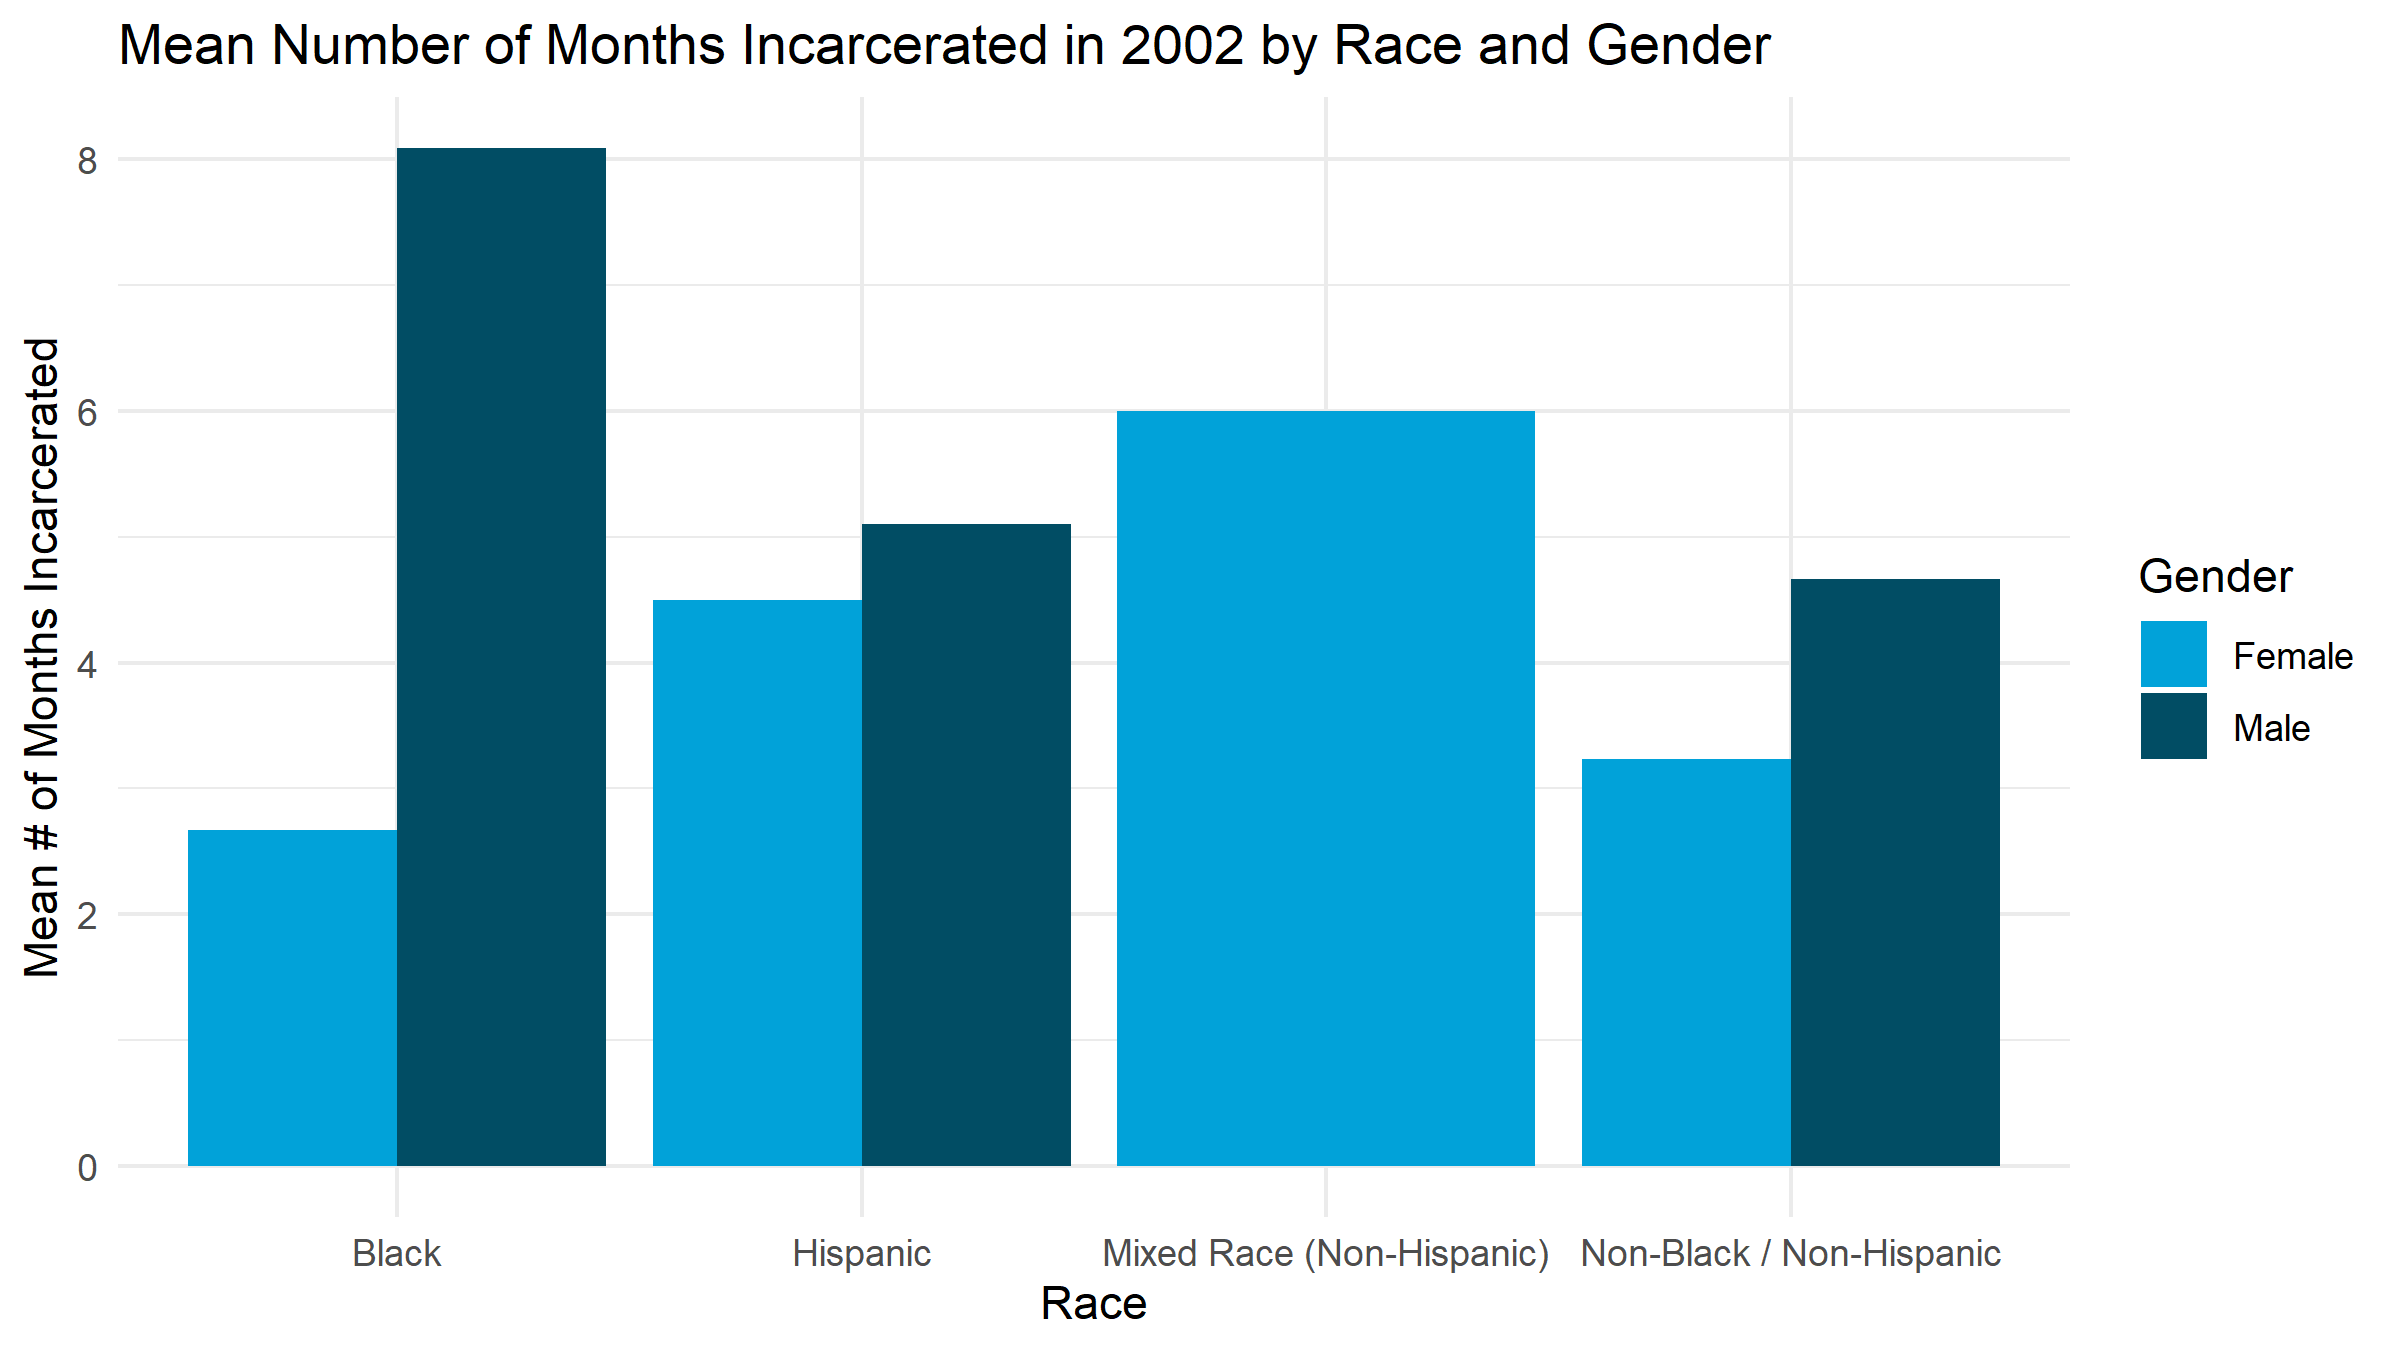
\includegraphics[width=.85\textwidth]{incarceration_by_racegender.png}
    \end{center}
    \caption{Mean Number of Months Incarcerated in 2002 by Race and Gender}
    \label{fig:graph}
\end{figure}

Table \ref{tab:summarystats} shows the numbers associated with each bar in Figure \ref{fig:graph}. As we see in Table \ref{tab:summarystats_n}, once we select only individuals who were incarcerated, we have limited data on the Mixed Race Non Hispanic group, and generally less data points for females.

\begin{table}[H]

\caption{\label{tab:summarystats}Mean Number of Months Incarcerated in 2002 by Race and Gender}
\centering
\begin{tabular}[t]{lrrrr}
\toprule
Gender & Black & Hispanic & Mixed Race Non Hispanic & Non Black Non Hispanic\\
\midrule
\cellcolor{gray!6}{Female} & \cellcolor{gray!6}{2.666667} & \cellcolor{gray!6}{4.500000} & \cellcolor{gray!6}{6} & \cellcolor{gray!6}{3.230769}\\
Male & 8.090909 & 5.103448 & NA & 4.666667\\
\bottomrule
\end{tabular}
\end{table}


\begin{table}[H]

\caption{\label{tab:summarystats_n}Sample Size of Each Group}
\centering
\begin{tabular}[t]{lrrrr}
\toprule
Gender & Black & Hispanic & Mixed Race Non Hispanic & Non Black Non Hispanic\\
\midrule
\cellcolor{gray!6}{Female} & \cellcolor{gray!6}{9} & \cellcolor{gray!6}{6} & \cellcolor{gray!6}{1} & \cellcolor{gray!6}{13}\\
Male & 66 & 29 & NA & 54\\
\bottomrule
\end{tabular}
\end{table}


\newpage

\section{Regression Summary}
The results from our regression below show that incarcerated black males serve on average 2.61 months more time than incarcerated black females. Further, incarcerated non-black/Non-Hispanic females serve on average 2.8 months fewer than black females.
In order to analyze this further across different groups, I would want to test different linear combinations of these groups. Surprisingly, even with the limited sample size, we can have quite a few statistically significant coefficients which we can use for inference.

% Table created by stargazer v.5.2.2 by Marek Hlavac, Harvard University. E-mail: hlavac at fas.harvard.edu
% Date and time: Fri, Feb 18, 2022 - 2:13:26 PM
\begin{table}[!htbp] \centering 
  \caption{Regression Output. Omitted category is Black Females.} 
  \label{tab:regression} 
\begin{tabular}{@{\extracolsep{5pt}}lc} 
\\[-1.8ex]\hline 
\hline \\[-1.8ex] 
 & \multicolumn{1}{c}{\textit{Dependent variable:}} \\ 
\cline{2-2} 
\\[-1.8ex] & Months Incarcerated in 2002 \\ 
\hline \\[-1.8ex] 
 Hispanic & $-$2.306$^{***}$ \\ 
  & (0.824) \\ 
  & \\ 
 Mixed Race (Non-Hispanic) & 0.857 \\ 
  & (0.729) \\ 
  & \\ 
 Non-Black / Non-Hispanic & $-$2.859$^{***}$ \\ 
  & (0.658) \\ 
  & \\ 
 Male & 2.610$^{***}$ \\ 
  & (0.741) \\ 
  & \\ 
 Constant & 5.143$^{***}$ \\ 
  & (0.729) \\ 
  & \\ 
\hline \\[-1.8ex] 
Observations & 178 \\ 
R$^{2}$ & 0.161 \\ 
Adjusted R$^{2}$ & 0.142 \\ 
Residual Std. Error & 3.946 (df = 173) \\ 
F Statistic & 8.302$^{***}$ (df = 4; 173) \\ 
\hline 
\hline \\[-1.8ex] 
\textit{Note:}  & \multicolumn{1}{r}{$^{*}$p$<$0.1; $^{**}$p$<$0.05; $^{***}$p$<$0.01} \\ 
\end{tabular} 
\end{table} 


\end{document}
